% !TEX program = xelatex
% A survey written from the talk "The Hall--Paige Conjecture" in the series
% Combinatorial Methods for Algebraic Problems. The slides are in slides/.
%   TEXINPUTS=../../shared/latex//: latexmk -xelatex -outdir=build main.tex
\documentclass[english]{yupin-notes}
\usepackage{yp-figures}

\title{The Hall--Paige Conjecture\\[0.3em]\large Rainbow perfect matchings in Cayley tables}
\author{Yuxuan Lu}
\date{}

\begin{document}
\maketitle
\tableofcontents

\section{Introduction}\label{sec:intro}

The subject of this survey is a question about finite groups that began as a question about arranging officers in a square. It was answered in 2009 with the help of the classification of finite simple groups, and since then it has been answered again, twice, by purely combinatorial means. Along the way it became a question about rainbow perfect matchings, and that is the form in which most of the recent progress, and most of the open problems, are stated.

\topic{Euler's thirty-six officers}

In 1782 Euler~\cite{eul1782} posed the following problem.

\begin{problem}[Euler, 1782]\label{prob:euler}
Six regiments each send six officers, one of each of six ranks. Can the $36$ officers stand in a $6\times6$ square so that every row and every column contains one officer of each regiment and one officer of each rank?
\end{problem}

Euler found no arrangement. Smaller versions of the puzzle have solutions; a card puzzle from Ozanam's \emph{R\'ecr\'eations math\'ematiques}~\cite{oza1723} asks for the sixteen court cards to be laid out so that every row and every column contains each rank and each suit, and Figure~\ref{fig:cards} shows a solution.

\begin{figure}[ht]
\centering
\begin{tikzpicture}[every node/.style={font=\large},
      card/.style={draw, minimum size=9mm, inner sep=0pt, outer sep=0pt}]
    \def\S{$\spadesuit$}\def\C{$\clubsuit$}%
    \def\H{\textcolor{RainbowRed}{$\heartsuit$}}%
    \def\D{\textcolor{RainbowRed}{$\diamondsuit$}}%
    \foreach \i/\row in {0/{A\S,Q\C,J\H,K\D}, 1/{K\H,J\D,Q\S,A\C},
                         2/{Q\D,A\H,K\C,J\S}, 3/{J\C,K\S,A\D,Q\H}}{%
      \foreach \c [count=\j] in \row
        \node[card] at (0.9*\j, -0.9*\i) {\c};}
  \end{tikzpicture}

\caption{A solution of Ozanam's card puzzle (1723): every row and every column contains each rank and each suit.}
\label{fig:cards}
\end{figure}

Such an arrangement is two squares in one. Forgetting the suits leaves a square of ranks in which every rank occurs once in each row and each column, and forgetting the ranks leaves a square of suits with the same property (Figure~\ref{fig:card-split}). Euler wrote the regiments with Latin letters and the ranks with Greek letters, which is where the name \emph{Latin square} comes from~\cite{mon24}.

\begin{figure}[ht]
\centering
\begin{tikzpicture}[every node/.style={font=\normalsize},
      cell/.style={draw, minimum size=7mm, inner sep=0pt, outer sep=0pt}]
    \def\S{$\spadesuit$}\def\C{$\clubsuit$}%
    \def\H{\textcolor{RainbowRed}{$\heartsuit$}}%
    \def\D{\textcolor{RainbowRed}{$\diamondsuit$}}%
    % the cards
    \foreach \i/\row in {0/{A\S,Q\C,J\H,K\D}, 1/{K\H,J\D,Q\S,A\C},
                         2/{Q\D,A\H,K\C,J\S}, 3/{J\C,K\S,A\D,Q\H}}{%
      \foreach \c [count=\j] in \row
        \node[cell] at (0.7*\j, -0.7*\i) {\c};}
    \node[font=\footnotesize] at (1.75,-3.0) {the cards};
    \node at (3.75,-1.05) {$=$};
    % the ranks
    \begin{scope}[shift={(4.2,0)}]
      \foreach \i/\row in {0/{A,Q,J,K}, 1/{K,J,Q,A}, 2/{Q,A,K,J}, 3/{J,K,A,Q}}{%
        \foreach \c [count=\j] in \row
          \node[cell] at (0.7*\j, -0.7*\i) {\c};}
      \node[font=\footnotesize] at (1.75,-3.0) {the ranks};
    \end{scope}
    \node at (7.95,-1.05) {$+$};
    % the suits
    \begin{scope}[shift={(8.4,0)}]
      \foreach \i/\row in {0/{\S,\C,\H,\D}, 1/{\H,\D,\S,\C},
                           2/{\D,\H,\C,\S}, 3/{\C,\S,\D,\H}}{%
        \foreach \c [count=\j] in \row
          \node[cell] at (0.7*\j, -0.7*\i) {\c};}
      \node[font=\footnotesize] at (1.75,-3.0) {the suits};
    \end{scope}
  \end{tikzpicture}

\caption{Forgetting the suits leaves a Latin square of ranks; forgetting the ranks leaves a Latin square of suits. Every rank--suit pair occurs exactly once.}
\label{fig:card-split}
\end{figure}

\begin{definition}\label{def:latin}
A \term{Latin square} of order $n$ is an $n\times n$ array of $n$ symbols in which every symbol occurs once in each row and once in each column. Two Latin squares $A=(a_{ij})$ and $B=(b_{ij})$ of order $n$ are \term{orthogonal} if the $n^2$ pairs $(a_{ij},b_{ij})$ are all distinct.
\end{definition}

Euler's problem asks for two orthogonal Latin squares of order $6$. He conjectured that this, and more, is impossible.

\begin{conjecture}[Euler, 1782]\label{conj:euler}
For $n\equiv2\pmod4$ there are no two orthogonal Latin squares of order $n$.
\end{conjecture}

For $n=2$ this is trivially true, and Tarry~\cite{tar1900} showed in 1900 that it is true for $n=6$: the thirty-six officers cannot be arranged. Beyond that Euler was wrong. Bose and Shrikhande~\cite{bs59} found counterexamples for $n=22$ and $n=50$ in 1959, and Bose, Shrikhande and Parker~\cite{bsp60} found counterexamples for every $n\equiv2\pmod4$ with $n\geq10$ in 1960. So the conjecture holds only for $n=2$ and $n=6$.

\topic{Latin squares in field trials}

Latin squares are also a tool of experimental design. R.~A.~Fisher promoted them in his experiments at Rothamsted between 1919 and 1933 and in \emph{The Design of Experiments} (1935); see Bailey~\cite{bai13}. The reason for balancing rows \emph{and} columns is the shape of a field. In Fisher's words, quoted by Bailey, ``on any given field agricultural operations \dots\ have followed one of two directions \dots; consequently streaks of fertility, weed infestation, etc., do, in fact, occur predominantly in those two directions'' (Fisher to Jeffreys, 1938). The oldest known example, again from Bailey, is an experiment on sixteen sheep by Cretté de Palluel in 1790 (Figure~\ref{fig:sheep}): the rows are slaughter dates, the columns are breeds, and the entries are diets, each diet occurring once on each date and once in each breed.

\begin{figure}[ht]
\centering
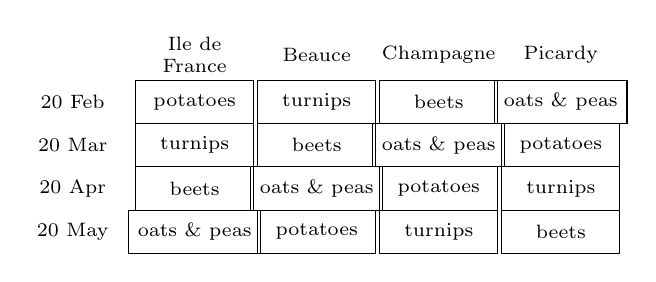
\begin{tikzpicture}[every node/.style={font=\scriptsize}]
    \foreach \b [count=\j] in {Ile de France,Beauce,Champagne,Picardy}
      \node[align=center, text width=1.45cm] at (1.55*\j,0.05) {\b};
    \foreach \d [count=\i] in {20 Feb,20 Mar,20 Apr,20 May}
      \node at (0,-0.55*\i) {\d};
    \foreach \row [count=\i] in {{potatoes,turnips,beets,oats \& peas},
                                 {turnips,beets,oats \& peas,potatoes},
                                 {beets,oats \& peas,potatoes,turnips},
                                 {oats \& peas,potatoes,turnips,beets}}
      \foreach \c [count=\j] in \row
        \node[draw, minimum width=1.5cm, minimum height=0.55cm] at (1.55*\j,-0.55*\i) {\c};
  \end{tikzpicture}

\caption{Cretté de Palluel's experiment of 1790 on sixteen sheep~\cite{bai13}. Rows: slaughter date; columns: breed; entries: diet.}
\label{fig:sheep}
\end{figure}

Superimposing a second square orthogonal to the first balances a second family of treatments against the rows, the columns and the first family. In the statistics literature such pairs are called \term{Graeco-Latin squares}~\cite{dey17}; Euler's nine officers of three regiments and three ranks (Figure~\ref{fig:nine-officers}) are the smallest interesting example. For odd orders they are easy to write down.

\begin{figure}[ht]
\centering
\begin{tikzpicture}[every node/.style={font=\small}]
    \foreach \row [count=\i] in {{A\alpha,B\beta,C\gamma},{C\beta,A\gamma,B\alpha},{B\gamma,C\alpha,A\beta}}
      \foreach \c [count=\j] in \row
        \node[lscell, minimum size=7.5mm] at (0.75*\j,-0.75*\i) {$\c$};
  \end{tikzpicture}

\caption{Nine officers: each Latin letter meets each Greek letter exactly once~\cite{bai13}.}
\label{fig:nine-officers}
\end{figure}

\begin{proposition}[see~\cite{bai13}]\label{prop:odd-pair}
For odd $n$, the Latin squares $L_1(i,j)=i+j$ and $L_2(i,j)=i-j$ on $\Z_n$ are orthogonal.
\end{proposition}

\begin{proof}
If the cells $(i_1,j_1)$ and $(i_2,j_2)$ carry the same pair, then $i_1+j_1=i_2+j_2$ and $i_1-j_1=i_2-j_2$, so $2(j_1-j_2)=0$. As $n$ is odd, $j_1=j_2$, and then $i_1=i_2$.
\end{proof}

The square $L_1$ is the addition table of $\Z_n$, so odd cyclic groups give orthogonal pairs at once. The difficulty lies in even orders, and it is there that the structure of the group begins to matter.

\section{From Latin squares to rainbow matchings}\label{sec:rainbow}

Euler's question is about a pair of Latin squares, but it can be rephrased as a question about one. The key notion is that of a transversal.

\begin{definition}\label{def:transversal}
A \term{transversal} of a Latin square of order $n$ is a set of $n$ cells, one in each row and one in each column, containing $n$ distinct symbols.
\end{definition}

In Ozanam's puzzle the four cells holding the spades form a transversal of the square of ranks, and so do the cells of each of the other suits. The four suits therefore split the square of ranks into four disjoint transversals (Figure~\ref{fig:suit-transversals}). This is a general fact; see Wanless's survey~\cite{wan07}.

\begin{figure}[ht]
\centering
\begin{tikzpicture}[every node/.style={font=\large},
      cell/.style={draw, minimum size=10mm, inner sep=0pt, outer sep=0pt}]
    \colorlet{suitS}{RainbowBlue!35}\colorlet{suitH}{RainbowRed!35}%
    \colorlet{suitD}{RainbowAmber!45}\colorlet{suitC}{RainbowGreen!40}%
    \foreach \i/\row in {0/{A/S,Q/C,J/H,K/D}, 1/{K/H,J/D,Q/S,A/C},
                         2/{Q/D,A/H,K/C,J/S}, 3/{J/C,K/S,A/D,Q/H}}{%
      \foreach \r/\u [count=\j] in \row
        \node[cell, fill=suit\u] at (1.0*\j, -1.0*\i) {\r};}
    \foreach \u/\sym/\y in {S/{$\spadesuit$}/0, H/{\textcolor{RainbowRed}{$\heartsuit$}}/-1,
                            D/{\textcolor{RainbowRed}{$\diamondsuit$}}/-2, C/{$\clubsuit$}/-3}{%
      \node[cell, fill=suit\u, minimum size=6mm] at (5.4,\y) {};
      \node[anchor=west, font=\normalsize] at (5.8,\y) {\sym};}
  \end{tikzpicture}

\caption{The ranks, shaded by suit. Each suit picks one cell in every row, every column and every rank.}
\label{fig:suit-transversals}
\end{figure}

\topic{The dictionary}

A Latin square $L$ of order $n$ can be read as an edge colouring of the complete bipartite graph $K_{n,n}$: the vertices on one side are the rows, the vertices on the other side are the columns, and the edge joining row $i$ to column $j$ receives the colour $L(i,j)$. The colouring is \term{proper}, meaning that edges sharing a vertex have different colours, precisely because each symbol occurs once in each row and once in each column. Conversely every proper $n$-edge-colouring of $K_{n,n}$ arises from a Latin square in this way. A transversal is then a perfect matching whose edges have distinct colours, that is, a \term{rainbow perfect matching} (Figure~\ref{fig:ranks-knn}).

\begin{figure}[ht]
\centering
\begin{tikzpicture}[every node/.style={font=\normalsize},
      cell/.style={draw, minimum size=7.6mm, inner sep=0pt, outer sep=0pt}]
    \def\cA{RainbowRed}\def\cK{RainbowBlue}\def\cQ{RainbowGreen}\def\cJ{black}%
    \foreach \i/\row in {1/{A,Q,J,K}, 2/{K,J,Q,A}, 3/{Q,A,K,J}, 4/{J,K,A,Q}}{%
      \node[font=\footnotesize] at (0.2, -0.76*\i) {$\i$};
      \foreach \r [count=\j] in \row
        \node[cell] at (0.76*\j, -0.76*\i) {\textcolor{\csname c\r\endcsname}{\r}};}
    \foreach \j in {1,...,4} \node[font=\footnotesize] at (0.76*\j, -0.2) {$\j$};
    \node[font=\footnotesize, anchor=east] at (0.05, -0.2) {row\,\textbackslash\,col};
    \foreach \i/\j in {1/1, 2/3, 3/4, 4/2}
      \node[circled, minimum size=6.4mm] at (0.76*\j, -0.76*\i) {};
    \node at (4.45,-1.9) {$\Longleftrightarrow$};
    \begin{scope}[shift={(5.6,0)}]
      \node[font=\footnotesize] at (0,-0.2) {rows};
      \node[font=\footnotesize] at (2.6,-0.2) {columns};
      \foreach \i in {1,...,4}{%
        \node[bvertex] (L\i) at (0,-0.76*\i) {};
        \node[bvertex] (R\i) at (2.6,-0.76*\i) {};
        \node[left=3pt of L\i, font=\footnotesize] {$\i$};
        \node[right=3pt of R\i, font=\footnotesize] {$\i$};}
      \foreach \i/\row in {1/{A,Q,J,K}, 2/{K,J,Q,A}, 3/{Q,A,K,J}, 4/{J,K,A,Q}}{%
        \foreach \r [count=\j] in \row
          \draw[\csname c\r\endcsname, opacity=.35] (L\i) -- (R\j);}
      \foreach \i/\j/\r in {1/1/A, 2/3/Q, 3/4/J, 4/2/K}
        \draw[\csname c\r\endcsname, line width=2.2pt] (L\i) -- (R\j);
      \node[align=left, font=\footnotesize, anchor=west] at (3.3,-1.9)
        {edge $ij$ gets the\\ colour of cell $(i,j)$:\\[2pt]
         \textcolor{RainbowRed}{A}, \textcolor{RainbowBlue}{K},
         \textcolor{RainbowGreen}{Q}, J};
    \end{scope}
  \end{tikzpicture}

\caption{The ranks as a proper colouring of $K_{4,4}$; the circled transversal is the bold rainbow perfect matching.}
\label{fig:ranks-knn}
\end{figure}

\begin{center}
\renewcommand{\arraystretch}{1.3}
\begin{tabular}{rcl}
Latin square of order $n$ & $\longleftrightarrow$ & proper $n$-edge-colouring of $K_{n,n}$\\
transversal & $\longleftrightarrow$ & rainbow perfect matching\\
orthogonal mate & $\longleftrightarrow$ & decomposition into $n$ rainbow perfect matchings
\end{tabular}
\end{center}

The last line of this dictionary is the content of the following proposition.

\begin{proposition}[cf.~\cite{wan07}]\label{prop:mate}
For a Latin square $L$ of order $n$ the following are equivalent:
\begin{enumerate}
\item $L$ has an orthogonal mate;
\item the cells of $L$ split into $n$ disjoint transversals;
\item the edges of $K_{n,n}$, coloured by $L$, split into $n$ rainbow perfect matchings.
\end{enumerate}
\end{proposition}

\begin{proof}
Suppose $M$ is an orthogonal mate of $L$ and fix a symbol $s$. The $n$ cells with $M=s$ lie in distinct rows and distinct columns, as $M$ is Latin, and they carry distinct $L$-symbols, as the pairs $(L,M)$ are distinct. So they form a transversal of $L$, and different symbols $s$ give disjoint transversals. Conversely, given $n$ disjoint transversals, number them $1,\dots,n$ and let $M(i,j)$ be the number of the transversal containing $(i,j)$. Each row and each column meets each transversal once, so $M$ is Latin, and transversal $s$ contains each symbol $a$ of $L$ exactly once, so the pair $(a,s)$ occurs exactly once. The equivalence of the last two statements is the dictionary: a transversal is a rainbow perfect matching.
\end{proof}

\topic{Does one rainbow perfect matching exist?}

Euler asked for a decomposition into rainbow perfect matchings, but even one need not exist; we will see in Section~\ref{sec:complete-mappings} that the addition table of $\Z_4$ has none. The natural conjecture is that one can always come within one cell.

\begin{conjecture}[Ryser--Brualdi--Stein; Ryser~\cite{rys67}, Stein~\cite{ste75}]\label{conj:rbs}
Every Latin square of order $n$ has a partial transversal with $n-1$ cells, and a transversal if $n$ is odd.
\end{conjecture}

Montgomery~\cite{mon23} proved that for all large $n$ every Latin square of order $n$ has a partial transversal with $n-1$ cells, so the conjecture holds for large even $n$. The odd case, which asks for a full transversal, is open.

\section{Cayley tables and complete mappings}\label{sec:complete-mappings}

The most natural Latin squares come from groups.

\begin{definition}\label{def:cayley-table}
The \term{Cayley table} of a finite group $G$ has its rows and columns indexed by $G$ and the entry $ab$ in cell $(a,b)$. It is a Latin square. As a colouring of a complete bipartite graph, it is the graph $K_{G,G}$ whose two sides are copies of $G$, with the edge $(x,y)$ coloured $xy$.
\end{definition}

The square of ranks in Ozanam's puzzle is a Cayley table. Renaming the ranks A, Q, J, K as $00,01,10,11$ and labelling the rows $00,11,01,10$ and the columns $00,01,10,11$, every cell becomes the sum of its row label and its column label in $\Z_2\times\Z_2$, and no cell moves (Figure~\ref{fig:ranks-cayley}).

\begin{figure}[ht]
\centering
\begin{tikzpicture}[every node/.style={font=\normalsize},
      cell/.style={draw, minimum size=7mm, inner sep=0pt, outer sep=0pt}]
    \def\cA{RainbowRed}\def\cK{RainbowBlue}\def\cQ{RainbowGreen}\def\cJ{black}%
    \def\gA{00}\def\gQ{01}\def\gJ{10}\def\gK{11}%
    \foreach \i/\row in {1/{A,Q,J,K}, 2/{K,J,Q,A}, 3/{Q,A,K,J}, 4/{J,K,A,Q}}{%
      \foreach \r [count=\j] in \row
        \node[cell] at (0.7*\j, -0.7*\i) {\textcolor{\csname c\r\endcsname}{\r}};}
    \node[font=\footnotesize] at (1.75,-3.45) {the ranks};
    \node[align=center, font=\small] at (4.6,-1.75)
      {$\xrightarrow{\ \text{rename}\ }$\\[4pt]
       \textcolor{RainbowRed}{A}$\,\mapsto00$\quad \textcolor{RainbowGreen}{Q}$\,\mapsto01$\\
       J$\,\mapsto10$\quad \textcolor{RainbowBlue}{K}$\,\mapsto11$};
    \begin{scope}[shift={(6.3,0)}]
      \foreach \i/\x/\row in {1/00/{A,Q,J,K}, 2/11/{K,J,Q,A},
                              3/01/{Q,A,K,J}, 4/10/{J,K,A,Q}}{%
        \node[font=\footnotesize, text=CiteColor] at (-0.02, -0.7*\i) {$\x$};
        \foreach \r [count=\j] in \row
          \node[cell] at (0.7*\j, -0.7*\i)
            {\textcolor{\csname c\r\endcsname}{$\csname g\r\endcsname$}};}
      \foreach \y [count=\j] in {00,01,10,11}
        \node[font=\footnotesize, text=CiteColor] at (0.7*\j, -0.2) {$\y$};
      \node[font=\footnotesize] at (-0.02,-0.2) {$+$};
      \node[font=\footnotesize] at (1.75,-3.45)
        {the addition table of $\mathbb Z_2\times\mathbb Z_2$};
    \end{scope}
  \end{tikzpicture}

\caption{Renaming the ranks and labelling the rows and columns by elements of $\Z_2\times\Z_2$, every cell becomes row $+$ column.}
\label{fig:ranks-cayley}
\end{figure}

So we may ask which groups $G$ have a Cayley table that decomposes into transversals. For a group, one transversal is enough.

\begin{fact}\label{fact:translates}
Let $T=\{(x,\phi(x)):x\in G\}$ be a transversal of the Cayley table of $G$. For each $g\in G$ the set
\[
T_g=\{(x,\phi(x)g):x\in G\}
\]
is again a transversal, and the $|G|$ sets $T_g$ partition the table.
\end{fact}

The entries of $T_g$ are those of $T$ multiplied on the right by $g$; in Ozanam's puzzle the four suits are exactly the four translates of the spade transversal (Figure~\ref{fig:translates}). For a group, therefore, Euler's question asks for a single rainbow perfect matching.

\begin{figure}[ht]
\centering
\begin{tikzpicture}[every node/.style={font=\normalsize},
      cell/.style={draw, minimum size=8mm, inner sep=0pt, outer sep=0pt}]
    \colorlet{suitS}{RainbowBlue!35}\colorlet{suitH}{RainbowRed!35}%
    \colorlet{suitD}{RainbowAmber!45}\colorlet{suitC}{RainbowGreen!40}%
    \foreach \i/\x/\row in {1/00/{00/S,01/C,10/H,11/D}, 2/11/{11/H,10/D,01/S,00/C},
                            3/01/{01/D,00/H,11/C,10/S}, 4/10/{10/C,11/S,00/D,01/H}}{%
      \node[font=\footnotesize, text=CiteColor] at (0.0, -0.8*\i) {$\x$};
      \foreach \v/\u [count=\j] in \row
        \node[cell, fill=suit\u] at (0.8*\j, -0.8*\i) {$\v$};}
    \foreach \y [count=\j] in {00,01,10,11}
      \node[font=\footnotesize, text=CiteColor] at (0.8*\j, -0.2) {$\y$};
    \node[font=\footnotesize] at (0.0,-0.2) {$+$};
    \foreach \u/\sym/\g/\y in {S/{$\spadesuit$}/{$T$}/-0.8,
        H/{\textcolor{RainbowRed}{$\heartsuit$}}/{$T+10$}/-1.6,
        D/{\textcolor{RainbowRed}{$\diamondsuit$}}/{$T+11$}/-2.4,
        C/{$\clubsuit$}/{$T+01$}/-3.2}{%
      \node[cell, fill=suit\u, minimum size=5.5mm] at (4.3,\y) {};
      \node[anchor=west] at (4.65,\y) {\sym\ \ \g};}
  \end{tikzpicture}

\caption{The four suits are the translates of one transversal $T$, obtained by shifting every column label by the same element.}
\label{fig:translates}
\end{figure}

\topic{Mann's complete mappings}

By 1942 every known pair of orthogonal Latin squares, whether in the statistical tables of Fisher and Yates~\cite{fy} or constructed from Galois fields by Bose~\cite{bose38} and Stevens~\cite{ste39}, was based on a group. Mann~\cite{man42} asked which groups can be used, and introduced the following notion.

\begin{definition}[Mann~\cite{man42}]\label{def:complete-mapping}
A bijection $\theta\colon G\to G$ is a \term{complete mapping} if $x\mapsto x\,\theta(x)$ is also a bijection.
\end{definition}

In the Cayley table, a complete mapping chooses in row $x$ the cell in column $\theta(x)$; these $n$ cells form a transversal, and every transversal arises in this way.

\begin{theorem}[Mann~\cite{man42}; Paige~\cite{pai51}]\label{thm:mann}
The Cayley table of $G$ has an orthogonal mate if and only if $G$ has a complete mapping $\theta$. One mate is the Latin square $S(i,k)=i\,k\,\theta(k)$.
\end{theorem}

The translation to rainbow matchings is immediate.

\begin{proposition}\label{prop:cm}
A bijection $\theta\colon G\to G$ is a complete mapping if and only if the perfect matching $\{(x,\theta(x)):x\in G\}$ of $K_{G,G}$ is rainbow. Every rainbow perfect matching of $K_{G,G}$ arises in this way from exactly one $\theta$.
\end{proposition}

\begin{proof}
A perfect matching of $K_{G,G}$ is the graph of a bijection $\theta$. Its colours are the elements $x\theta(x)$, and these are distinct exactly when $x\mapsto x\theta(x)$ is injective, that is, a bijection.
\end{proof}

\begin{corollary}\label{cor:cm}
The following are equivalent: $G$ has a complete mapping; $K_{G,G}$ has a rainbow perfect matching; the edges of $K_{G,G}$ split into $|G|$ rainbow perfect matchings.
\end{corollary}

\begin{proof}
Combine Proposition~\ref{prop:cm} with Fact~\ref{fact:translates} and Proposition~\ref{prop:mate}.
\end{proof}

\topic{The first results}

The first results on complete mappings appeared between 1942 and 1951.
\begin{itemize}
\item Mann~\cite{man42} showed in 1942 that \emph{no group of order $4n+2$ has a complete mapping}, so groups can never refute Euler's conjecture. In the same paper he obtained new orthogonal pairs of order $12$, from $\Z_2\times\Z_2\times\Z_3$ and from $A_4$, beyond the reach of the Galois-field method.
\item Paige~\cite{pai47} showed in 1947 that an abelian group has a complete mapping if and only if $\sum_{x\in G}x=0$.
\item Bateman~\cite{bat50} showed in 1950 that every infinite group has a complete mapping.
\item Paige~\cite{pai51} showed in 1951 that every group of odd order has one, namely $\theta(x)=x$.
\end{itemize}
Paige also found a necessary condition for general groups.

\begin{theorem}[Paige~\cite{pai51}]\label{thm:paige}
If $G$ has a complete mapping, then the product of all elements of $G$, taken in any order, lies in the commutator subgroup $G'$.
\end{theorem}

Paige conjectured the converse. He also conjectured that no symmetric group $S_n$ has a complete mapping.

\begin{example}\label{ex:order-four}
The two groups of order $4$ already behave differently (Figure~\ref{fig:z2z2-z4}). In $\Z_2\times\Z_2$ we have $00+01+10+11=00$, so Paige's condition holds, and the Cayley table has a transversal. In $\Z_4$ we have $0+1+2+3=2\neq0$, so Paige's condition fails and the Cayley table has no transversal. The two tables are Latin squares of the same order; what separates them is the structure of the group.
\end{example}

\begin{figure}[ht]
\centering
\begin{tikzpicture}[every node/.style={font=\normalsize},
      cell/.style={draw, minimum size=7.5mm, inner sep=0pt, outer sep=0pt}]
    \def\cA{RainbowRed}\def\cK{RainbowBlue}\def\cQ{RainbowGreen}\def\cJ{black}%
    \def\gA{00}\def\gQ{01}\def\gJ{10}\def\gK{11}%
    \foreach \i/\x/\row in {1/00/{A,Q,J,K}, 2/11/{K,J,Q,A},
                            3/01/{Q,A,K,J}, 4/10/{J,K,A,Q}}{%
      \node[font=\footnotesize, text=CiteColor] at (0.0, -0.75*\i) {$\x$};
      \foreach \r [count=\j] in \row
        \node[cell] at (0.75*\j, -0.75*\i)
          {\textcolor{\csname c\r\endcsname}{$\csname g\r\endcsname$}};}
    \foreach \y [count=\j] in {00,01,10,11}
      \node[font=\footnotesize, text=CiteColor] at (0.75*\j, -0.2) {$\y$};
    \node[font=\footnotesize] at (0.0,-0.2) {$+$};
    \foreach \i/\j in {1/1, 2/3, 3/4, 4/2}
      \node[circled, minimum size=6.6mm] at (0.75*\j, -0.75*\i) {};
    \node at (1.875,-3.85) {$\mathbb Z_2\times\mathbb Z_2$};
    \begin{scope}[shift={(5.2,0)}]
      \foreach \i in {0,...,3}{%
        \node[font=\footnotesize, text=CiteColor] at (0.0, -0.75*\i-0.75) {$\i$};
        \node[font=\footnotesize, text=CiteColor] at (0.75*\i+0.75, -0.2) {$\i$};
        \foreach \j in {0,...,3}{%
          \pgfmathtruncatemacro{\v}{mod(\i+\j,4)}%
          \node[cell] at (0.75*\j+0.75, -0.75*\i-0.75) {$\v$};}}
      \node[font=\footnotesize] at (0.0,-0.2) {$+$};
      \node at (1.875,-3.85) {$\mathbb Z_4$};
    \end{scope}
  \end{tikzpicture}

\caption{The Cayley tables of $\Z_2\times\Z_2$ and $\Z_4$. The first has a transversal (circled); the second has none.}
\label{fig:z2z2-z4}
\end{figure}

\topic{Hall and Paige, 1955}

Hall and Paige~\cite{hp55} translated Paige's condition into a statement about Sylow subgroups.

\begin{fact}[Hall--Paige~\cite{hp55}]\label{fact:sylow}
The product of all elements of $G$ lies in $G'$ if and only if the Sylow $2$-subgroups of $G$ are trivial or non-cyclic.
\end{fact}

For $\Z_4$ the Sylow $2$-subgroup is $\Z_4$ itself, which is cyclic; for $\Z_2\times\Z_2$ it is not. In the same paper Hall and Paige proved that every \emph{solvable} group with this property has a complete mapping, and that $S_n$ for $n>3$ and $A_n$ have complete mappings, so Paige's conjecture on symmetric groups was false. They conjectured the converse of Theorem~\ref{thm:paige} in the following form.

\begin{conjecture}[Hall--Paige~\cite{hp55}]\label{conj:hp}
A finite group $G$ has a complete mapping if and only if its Sylow $2$-subgroups are trivial or non-cyclic.
\end{conjecture}

We say that $G$ satisfies the \term{Hall--Paige condition} if its Sylow $2$-subgroups are trivial or non-cyclic.

\section{Three proofs of the Hall--Paige conjecture}\label{sec:proof}

\topic{The proof via the classification}

The first proof was completed in 2009 and runs through the classification of finite simple groups.
\begin{itemize}
\item Hall and Paige~\cite{hp55} showed that if a normal subgroup $N$ of $G$ and the quotient $G/N$ both have complete mappings, then so does $G$. This settles the solvable case.
\item Wilcox~\cite{wil09} showed that a minimal counterexample is simple, and handled the groups of Lie type uniformly. This left the Tits group and the $26$ sporadic groups.
\item Evans~\cite{eva09} treated all of these except the fourth Janko group $J_4$, with computer algebra.
\item Bray treated $J_4$ in 2009; the proof was published in 2020 in~\cite{bccsz20}.
\end{itemize}

\begin{theorem}[Wilcox~\cite{wil09}, Evans~\cite{eva09}, Bray~\cite{bccsz20}, 2009]\label{thm:hp}
The Hall--Paige conjecture is true.
\end{theorem}

A question about Latin squares was thus settled by the classification of finite simple groups.

\topic{A proof by counting}

Eberhard, Manners and Mrazovi\'c~\cite{emm22} gave a second proof, for large groups, by counting complete mappings. We write $G^{ab}$ for the abelianisation $G/G'$.

\begin{theorem}[Eberhard--Manners--Mrazovi\'c~\cite{emm22}]\label{thm:emm}
If $G$ has order $n$ and satisfies the Hall--Paige condition, then the number of complete mappings of $G$ is
\[
\bigl(e^{-1/2}+o(1)\bigr)\,|G^{ab}|\,\frac{n!^2}{n^n}.
\]
\end{theorem}

The factor $n!\cdot n!/n^n$ is the naive guess: there are $n!$ bijections $\phi$, and $x\mapsto x\phi(x)$ is a bijection with ``probability'' $n!/n^n$. Since the count is positive for every large $G$, Theorem~\ref{thm:emm} proves the Hall--Paige conjecture for large groups without the classification, though not by a construction. Combined with Wilcox's reduction, only the Mathieu groups $M_{11}$ and $M_{12}$ need to be treated separately.

\topic{A proof by random subsets}

The third approach keeps only part of the Cayley table. Take sets $X$ of rows, $Y$ of columns and $Z$ of symbols with $|X|=|Y|=|Z|$; a transversal of what is left uses every symbol of $Z$ exactly once.

\begin{fact}\label{fact:sum}
If such a transversal exists, then $\sum X+\sum Y=\sum Z$ in $G^{ab}$.
\end{fact}

This is the same sum argument as for the Hall--Paige condition. M\"uyesser and Pokrovskiy showed that, for sets that look random, nothing else is needed.

\begin{theorem}[M\"uyesser--Pokrovskiy~\cite{mp25a}]\label{thm:random-hp}
Let $G$ be large. If $X,Y,Z$ are each close to a random subset of $G$, in which every element is kept independently with probability $p$, then $\sum X+\sum Y=\sum Z$ in $G^{ab}$ is also sufficient for the existence of a transversal.
\end{theorem}

Taking $X=Y=Z=G$, that is $p=1$, gives the Hall--Paige conjecture for large $G$, again with no use of the classification.

\topic{The dictionary}

We collect the translations used so far, together with those of the later sections.

\begin{center}
\renewcommand{\arraystretch}{1.25}
\small
\begin{tabular}{p{0.42\textwidth}p{0.5\textwidth}}
\textbf{algebra / Latin squares} & \textbf{graphs}\\\hline
Latin square of order $n$ & proper $n$-edge-colouring of $K_{n,n}$\\
transversal & rainbow perfect matching\\
orthogonal mate & decomposition into $n$ rainbow perfect matchings\\
Cayley table of $G$ & $K_{G,G}$, edge $(x,y)$ coloured $xy$\\
complete mapping of $G$ & rainbow perfect matching of $K_{G,G}$\\
number of complete mappings & number of rainbow perfect matchings\\
strong complete mapping & perfect matching rainbow in two colourings\\
transversal of a subsquare $A\times B$ & rainbow perfect matching of $K_{A,B}$\\
orthomorphism with a given cycle type & rainbow cycle factor in $\operatorname{Cay}(G,G\setminus\{e\})$
\end{tabular}
\end{center}

Beyond the Hall--Paige conjecture three questions suggest themselves, and the rest of this survey is organised around them. \emph{How many} transversals does a Cayley table have, and which groups have the most (Section~\ref{sec:counting})? \emph{In which subsets}: if we delete some rows, columns and symbols, when does what is left still have a transversal (Section~\ref{sec:subsquares})? \emph{Of which shape}: a complete mapping is a permutation of $G$, so which cycle types can it have (Section~\ref{sec:cycle-types})?

\section{How many transversals? Semiqueens and queens}\label{sec:counting}

\topic{Counting complete mappings}

The first result on the number of transversals concerned cyclic groups and was conjectured by Vardi.

\begin{theorem}[Eberhard--Manners--Mrazovi\'c~\cite{emm19}; Vardi's conjecture]\label{thm:emm19}
For odd $n$, the Cayley table of $\Z_n$ has
\[
\bigl(e^{-1/2}+o(1)\bigr)\,n\,\frac{n!^2}{n^n}
\]
transversals.
\end{theorem}

Equivalently, this counts the ways to place $n$ non-attacking \term{semiqueens} on an $n\times n$ board wrapped into a torus; a semiqueen moves along rows, columns and one family of diagonals. Vardi~\cite{var91} conjectured in 1991 that the count lies between $c_1^n\,n!$ and $c_2^n\,n!$ for constants $0<c_1\leq c_2<1$, the lower bound being the hard part. Theorem~\ref{thm:emm} extends Theorem~\ref{thm:emm19} to every group, with the same constant $e^{-1/2}$ and an extra factor $|G^{ab}|$, and has the following consequence.

\begin{corollary}[Eberhard--Manners--Mrazovi\'c~\cite{emm22}]\label{cor:most}
For large $k$, among all groups of order $2^k$, the elementary abelian group $\Z_2^k$ has the most complete mappings.
\end{corollary}

\topic{The $n$-queens problem}

The semiqueens are a relative of a much older puzzle.

\begin{problem}[Bezzel~\cite{bez1848}, 1848]\label{prob:queens}
Place eight queens on a chessboard so that no two attack each other, that is, no two share a row, a column or a diagonal.
\end{problem}

Nauck~\cite{nau1850} found all $92$ solutions in 1850; Gauss also worked on the puzzle. Pauls~\cite{pau1874} showed in 1874 that on an $n\times n$ board $n$ non-attacking queens fit for every $n\notin\{2,3\}$. Let $Q(n)$ denote the number of solutions, so that $Q(8)=92$; the question is how $Q(n)$ grows.

\begin{figure}[ht]
\centering
\begin{tikzpicture}[scale=0.42]
    \foreach \i in {0,...,7}{\foreach \j in {0,...,7}{%
      \pgfmathtruncatemacro{\pty}{mod(\i+\j,2)}%
      \ifnum\pty=1 \fill[black!12] (\j,-\i) rectangle ++(1,-1);\fi}}
    \draw (0,0) rectangle (8,-8);
    \foreach \c [count=\r from 0] in {1,5,8,6,3,7,2,4}
      \fill[BlkConjecture] (\c-0.5,-\r-0.5) circle (0.3);
  \end{tikzpicture}

\caption{A solution of the eight-queens puzzle.}
\label{fig:eight-queens}
\end{figure}

Number the rows and the columns $1,\dots,n$. With one queen in each row and each column, the queen of row $j$ stands in column $\sigma(j)$ for a permutation $\sigma$, and the square $(j,c)$ lies on the diagonals $c+j=\text{const}$ and $c-j=\text{const}$.

\begin{fact}\label{fact:queens}
A permutation $\sigma$ is a solution if and only if the $n$ numbers $\sigma(j)+j$ are distinct and the $n$ numbers $\sigma(j)-j$ are distinct.
\end{fact}

For the solution in Figure~\ref{fig:eight-queens}:
\begin{center}
\renewcommand{\arraystretch}{1.2}
\begin{tabular}{r|cccccccc}
$j$ & 1&2&3&4&5&6&7&8\\\hline
$\sigma(j)$ & 1&5&8&6&3&7&2&4\\
$\sigma(j)+j$ & 2&7&11&10&8&13&9&12\\
$\sigma(j)-j$ & 0&3&5&2&$-2$&1&$-5$&$-4$
\end{tabular}
\end{center}

\topic{P\'olya's toroidal board}

P\'olya~\cite{pol1918} studied in 1918 the \emph{doubly periodic} solutions: those that remain non-attacking when the board is repeated to fill the whole plane (Figure~\ref{fig:queens-tiled}). Equivalently the diagonals wrap around, the board is a torus, and the numbers $\sigma(j)+j$ and $\sigma(j)-j$ must be distinct modulo $n$. The torus is the more regular problem, with $n$ rows, $n$ columns and $n$ diagonals in each direction. A toroidal solution is also an ordinary one, so the number $T(n)$ of toroidal solutions satisfies $T(n)\leq Q(n)$, and P\'olya showed that $T(n)>0$ if and only if $n\equiv1,5\pmod6$.

\begin{figure}[ht]
\centering
\begin{tikzpicture}[scale=0.3]
    \foreach \bx in {0,1}{\foreach \by in {0,1}{%
      \foreach \i in {0,...,4}{\foreach \j in {0,...,4}{%
        \pgfmathtruncatemacro{\pty}{mod(\i+\j,2)}%
        \ifnum\pty=0 \fill[black!8] (5*\bx+\j,-5*\by-\i) rectangle ++(1,-1);\fi}}
      \foreach \j in {0,...,4}{%
        \pgfmathtruncatemacro{\c}{mod(2*\j,5)}%
        \fill[BlkConjecture] (5*\bx+\c+0.5,-5*\by-\j-0.5) circle (0.32);}}}
    \draw[step=1, black!30] (0,0) grid (10,-10);
    \draw[very thick] (0,0) rectangle (10,-10);
    \draw[very thick] (5,0) -- (5,-10) (0,-5) -- (10,-5);
  \end{tikzpicture}

\caption{Five queens on the $5\times5$ torus, repeated periodically: still no attacks.}
\label{fig:queens-tiled}
\end{figure}

On the torus, both puzzles are statements about the group $\Z_n$:
\begin{center}
\renewcommand{\arraystretch}{1.4}
\begin{tabular}{lll}
\textbf{on the $n\times n$ torus} & \textbf{condition on $\sigma$ (mod $n$)} & \textbf{in the group $\Z_n$}\\\hline
$n$ semiqueens & $\sigma(j)+j$ distinct & a complete mapping\\
$n$ queens & $\sigma(j)+j$ and $\sigma(j)-j$ distinct & a strong complete mapping
\end{tabular}
\end{center}
Semiqueens exist if and only if $n$ is odd, which is the Hall--Paige conjecture for $\Z_n$; queens exist if and only if $n\equiv1,5\pmod6$, by P\'olya's theorem. In Figure~\ref{fig:toroidal-queens}, where $\sigma(j)=2j$ on $\Z_5$, both $\sigma(j)+j=3j$ and $\sigma(j)-j=j$ are bijections of $\Z_5$.

\begin{figure}[ht]
\centering
\begin{tikzpicture}[scale=0.62]
    \foreach \i in {0,...,4}{\foreach \j in {0,...,4}{%
      \pgfmathtruncatemacro{\pty}{mod(\i+\j,2)}%
      \ifnum\pty=0 \fill[black!8] (\j,-\i) rectangle ++(1,-1);\fi}}
    \draw (0,0) grid (5,-5);
    \foreach \j in {0,...,4}{%
      \pgfmathtruncatemacro{\c}{mod(2*\j,5)}%
      \fill[BlkConjecture] (\c+0.5,-\j-0.5) circle (0.3);
      \node[font=\scriptsize, text=CiteColor] at (-0.4,-\j-0.5) {$\j$};
      \node[font=\scriptsize, text=CiteColor] at (\j+0.5,0.4) {$\j$};}
  \end{tikzpicture}

\caption{Five non-attacking queens on the $5\times5$ torus: $\sigma(j)=2j$ on $\Z_5$.}
\label{fig:toroidal-queens}
\end{figure}

\topic{Counting queens}

Rivin, Vardi and Zimmermann~\cite{rvz94} conjectured in 1994 that $\log Q(n)$ and $\log T(n)$ are both $\Theta(n\log n)$. Luria~\cite{lur17} showed that $T(n)\leq\bigl((1+o(1))\,ne^{-3}\bigr)^n$ and conjectured that this is tight. Bowtell and Keevash~\cite{bk21} proved that $T(n)=\bigl((1+o(1))\,ne^{-3}\bigr)^n$ for $n\equiv1,5\pmod6$, and Luria and Simkin~\cite{ls21} and Bowtell and Keevash~\cite{bk21} showed that $Q(n)\geq\bigl((1-o(1))\,ne^{-3}\bigr)^n$. Finally Simkin~\cite{sim21} determined the ordinary count:
\[
Q(n)=\bigl((1\pm o(1))\,ne^{-\alpha}\bigr)^n,\qquad \alpha=1.942\pm0.003,
\]
which is about $(0.143\,n)^n$. The tools are those of the Hall--Paige problem: a random greedy process, followed by absorption.

Two further results concern completion and symmetry.

\begin{theorem}[Glock--Munh\'a Correia--Sudakov~\cite{gms22}]\label{thm:completion}
For large $n$, any $n/60$ non-attacking queens on the $n\times n$ board can be completed to a solution, while some $\approx n/4$ non-attacking queens cannot.
\end{theorem}

The completion question goes back to Nauck~\cite{nau1850}, and the proof goes through rainbow matchings in bipartite graphs.

\begin{theorem}[Dai--Kelly~\cite{dk24}]\label{thm:reflecting}
For all large $n$ there is a reflecting $n$-queens configuration, answering questions of Klarner (1967) and Slater.
\end{theorem}

The group-theoretic generalisation of toroidal queens, strong complete mappings, is the subject of Problem~\ref{prob:strong}.

\section{In which subsets? Near transversals and subsquares}\label{sec:subsquares}

\topic{Deleting one row and one column}

A \term{near transversal} of a Latin square of order $n$ is a set of $n-1$ cells in distinct rows and distinct columns with distinct symbols. Since $\Z_{2m}$ has no transversal, $n-1$ is the best one can ask for in general.

\begin{theorem}[Goddyn--Halasz~\cite{gh20}]\label{thm:near}
Every Cayley table, and indeed every Latin square main-class equivalent to one, has a near transversal.
\end{theorem}

This is the Ryser--Brualdi--Stein conjecture for Cayley tables. In the language of Theorem~\ref{thm:random-hp}, the near transversal of $\Z_4$ in Figure~\ref{fig:z4-near} is a transversal for $X=G\setminus\{3\}$, $Y=G\setminus\{1\}$ and $Z=G\setminus\{2\}$, and indeed $\sum X+\sum Y=3+1=0=\sum Z$ in $\Z_4$. M\"uyesser and Pokrovskiy~\cite{mp25a} gave a second proof of Theorem~\ref{thm:near} for large groups in this way.

\begin{figure}[ht]
\centering
\begin{tikzpicture}[every node/.style={font=\normalsize},
      cell/.style={draw, minimum size=8mm, inner sep=0pt, outer sep=0pt}]
    \fill[black!10] (0.4,-2.8) rectangle (3.6,-3.6);
  \fill[black!10] (1.2,-0.4) rectangle (2.0,-3.6);
  \foreach \i/\j in {0/0, 1/2, 2/3}
    \draw[BlkConjecture, line width=1.6pt] (0.8*\j+0.8, -0.8*\i-0.8) circle (0.32);
    \foreach \i in {0,...,3}{%
      \node[font=\footnotesize, text=CiteColor] at (0.0, -0.8*\i-0.8) {$\i$};
      \node[font=\footnotesize, text=CiteColor] at (0.8*\i+0.8, -0.2) {$\i$};
      \foreach \j in {0,...,3}{%
        \pgfmathtruncatemacro{\v}{mod(\i+\j,4)}%
        \node[cell] at (0.8*\j+0.8, -0.8*\i-0.8) {$\v$};}}
    \node[font=\footnotesize] at (0.0,-0.2) {$+$};
  \end{tikzpicture}

\caption{The Cayley table of $\Z_4$ with row $3$, column $1$ and symbol $2$ deleted. The circled cells are a transversal of what is left.}
\label{fig:z4-near}
\end{figure}

\topic{Subsquares and Snevily's conjecture}

Keeping the rows in a set $A$ and the columns in a set $B$ with $|A|=|B|=k$ gives a $k\times k$ \term{subsquare} $A\times B$. In an abelian group, a transversal of it is a bijection $\pi\colon A\to B$ for which the $k$ sums $a+\pi(a)$ are distinct. Deleting rows and columns should only make a transversal easier to find, \emph{unless} what is left is itself the table of a group with no transversal (Figures~\ref{fig:z5-subsquare} and~\ref{fig:z4-subsquare}).

\begin{figure}[ht]
\centering
\begin{tikzpicture}[every node/.style={font=\normalsize},
      cell/.style={draw, minimum size=8mm, inner sep=0pt, outer sep=0pt}]
    \foreach \a [count=\i] in {0,1,3}{%
      \node[font=\footnotesize, text=CiteColor] at (0.0,-0.8*\i) {$\a$};
      \foreach \b [count=\j] in {0,2,4}{%
        \pgfmathtruncatemacro{\v}{mod(\a+\b,5)}%
        \node[cell] at (0.8*\j,-0.8*\i) {$\v$};}}
    \foreach \b [count=\j] in {0,2,4}
      \node[font=\footnotesize, text=CiteColor] at (0.8*\j,-0.2) {$\b$};
    \node[font=\footnotesize] at (0.0,-0.2) {$+$};
    \foreach \i/\j in {1/3, 2/1, 3/2}
      \draw[BlkConjecture, line width=1.6pt] (0.8*\j,-0.8*\i) circle (0.32);
  \end{tikzpicture}

\caption{The subsquare $\{0,1,3\}\times\{0,2,4\}$ of the Cayley table of $\Z_5$ has a transversal.}
\label{fig:z5-subsquare}
\end{figure}

\begin{figure}[ht]
\centering
\begin{tikzpicture}[every node/.style={font=\normalsize},
      cell/.style={draw, minimum size=8mm, inner sep=0pt, outer sep=0pt}]
    \foreach \i/\j in {0/0, 0/2, 2/0, 2/2}
    \fill[RainbowAmber!40] (0.8*\j+0.4, -0.8*\i-0.4) rectangle ++(0.8,-0.8);
    \foreach \i in {0,...,3}{%
      \node[font=\footnotesize, text=CiteColor] at (0.0, -0.8*\i-0.8) {$\i$};
      \node[font=\footnotesize, text=CiteColor] at (0.8*\i+0.8, -0.2) {$\i$};
      \foreach \j in {0,...,3}{%
        \pgfmathtruncatemacro{\v}{mod(\i+\j,4)}%
        \node[cell] at (0.8*\j+0.8, -0.8*\i-0.8) {$\v$};}}
    \node[font=\footnotesize] at (0.0,-0.2) {$+$};
  \end{tikzpicture}

\caption{The subsquare $\{0,2\}\times\{0,2\}$ of the Cayley table of $\Z_4$ is the table of $\Z_2$, and has no transversal.}
\label{fig:z4-subsquare}
\end{figure}

Snevily's note~\cite{sne99} contains four conjectures; the two below are his third and second, as combined by M\"uyesser and Pokrovskiy~\cite{mp25a}.

\begin{conjecture}[Snevily~\cite{sne99}]\label{conj:snevily}
Let $G$ be abelian and $A,B\subseteq G$ with $|A|=|B|$.
\begin{enumerate}
\item If $|G|$ is odd, then $A\times B$ has a transversal.
\item If $G\cong\Z_{2k}$, then $A\times B$ has a transversal unless $g_1+A=g_2+B=H$ for some cyclic subgroup $H$ of even order.
\end{enumerate}
\end{conjecture}

The first part says that in an abelian group of odd order \emph{every} subsquare has a transversal; for $k=|G|$ it is the odd case of the Hall--Paige conjecture, and Snevily notes that this case follows from a theorem of Hall~\cite{hall52}. The second part says that in $\Z_{2k}$ the only subsquares without a transversal are translates of the table of a cyclic subgroup of even order.

Progress on the first part was algebraic. Alon~\cite{alon00} proved it for $\Z_p$ by the Combinatorial Nullstellensatz, even when $A$ is a \emph{sequence} of $k<p$ elements with repetitions allowed. Dasgupta, K\'arolyi, Serra and Szegedy~\cite{dkss01} proved it for every cyclic group of odd order, and Arsovski~\cite{ars11} for every abelian group of odd order, by linear algebra over characters. There was no partial progress on the second part before 2025.

The second part cannot be stated for all abelian groups of even order, as the following example shows.

\begin{example}[Akbari--Alipour~\cite{aa04}]\label{ex:akbari-alipour}
In $G=\Z_2^k$ take $a_1\neq a_2$ and $b_1\neq b_2$ with $a_1+a_2+b_1+b_2=0$, and let $A=G\setminus\{a_1,a_2\}$ and $B=G\setminus\{b_1,b_2\}$. Then $A\times B$ has no transversal, although it is not the table of a subgroup.
\end{example}

\topic{All groups, large subsquares}

M\"uyesser and Pokrovskiy showed that for large subsquares these are the only obstructions, in every group.

\begin{theorem}[M\"uyesser--Pokrovskiy~\cite{mp25a}]\label{thm:subsquares}
Let $n$ be large, let $G$ be a group and let $A,B\subseteq G$ with $|A|=|B|=n$. Then $A\times B$ has a transversal unless, for some $g_1,g_2\in G$ and some subgroup $H\leq G$, one of the following holds:
\begin{enumerate}
\item $H$ fails the Hall--Paige condition, $A=g_1H$ and $B=Hg_2$;
\item $H\cong\Z_2^k$, $g_1A=H\setminus\{a_1,a_2\}$ and $g_2B=H\setminus\{b_1,b_2\}$ with $a_1+a_2+b_1+b_2=0$.
\end{enumerate}
\end{theorem}

In the first case $A\times B$ is a copy of the table of $H$, which has no transversal by the Hall--Paige theorem; the second case is the example of Akbari and Alipour. Nothing else goes wrong, and in particular both parts of Snevily's conjecture hold for large subsquares. Whether the same is true for every $n$ is Conjecture~\ref{conj:mp-every-n} below.

\section{Of which shape? Orthomorphisms and cycle types}\label{sec:cycle-types}

A complete mapping is a permutation of $G$, so it has a cycle type. It is more convenient to work with a closely related notion.

\begin{definition}\label{def:orthomorphism}
A bijection $\psi\colon G\to G$ is an \term{orthomorphism} if $x\mapsto x^{-1}\psi(x)$ is also a bijection. Equivalently, choosing in row $x$ of the Cayley table the cell with symbol $\psi(x)$ gives a transversal~\cite{wan07}.
\end{definition}

For example, the spade transversal of Ozanam's square, read as a permutation of $\Z_2\times\Z_2$, fixes $00$ and cycles $01\to10\to11\to01$ (Figure~\ref{fig:ortho-cycle}).

\begin{figure}[ht]
\centering
\begin{tikzpicture}[>=Latex, every node/.style={font=\normalsize}]
    \node[overtex, minimum size=8mm, inner sep=0pt] (e) at (0,0) {$00$};
    \draw[->, thick, BlkConjecture] (e) edge[loop above, looseness=6] (e);
    \node[overtex, minimum size=8mm, inner sep=0pt] (a) at (2.2,0.9) {$01$};
    \node[overtex, minimum size=8mm, inner sep=0pt] (b) at (3.5,-0.9) {$10$};
    \node[overtex, minimum size=8mm, inner sep=0pt] (c) at (0.9,-0.9) {$11$};
    \draw[->, thick, BlkConjecture] (a) to[bend left=20] (b);
    \draw[->, thick, BlkConjecture] (b) to[bend left=20] (c);
    \draw[->, thick, BlkConjecture] (c) to[bend left=20] (a);
  \end{tikzpicture}

\caption{The spade transversal as a permutation of $\Z_2\times\Z_2$.}
\label{fig:ortho-cycle}
\end{figure}

Prescribed cycle types have long-standing applications, as recorded by M\"uyesser~\cite{muy23}. A single cycle through all non-identity elements appears in Ringel's solution of the Heawood map-colouring problem, and orthomorphisms whose non-identity elements fall into disjoint $6$-cycles give cyclic Steiner triple systems.

\begin{conjecture}[Friedlander--Gordon--Tannenbaum~\cite{fgt81}]\label{conj:fgt}
Let $G$ be an abelian group of order $n$ satisfying the Hall--Paige condition, and let $k\geq2$ with $k\mid n-1$. Then some orthomorphism of $G$ fixes $0$ and permutes the other elements in disjoint $k$-cycles.
\end{conjecture}

Figure~\ref{fig:ortho-cycle} is the case $G=\Z_2\times\Z_2$, $k=3$. Friedlander, Gordon and Tannenbaum~\cite{fgt81} proved the conjecture for $|G|\leq15$ and for abelian $p$-groups with $p\geq3$. Even the case $k=3$ with $G$ cyclic remained open for forty years.

\begin{theorem}[M\"uyesser~\cite{muy23}]\label{thm:fgt}
The Friedlander--Gordon--Tannenbaum conjecture holds for all sufficiently large abelian groups.
\end{theorem}

\topic{Cycle types as rainbow cycle factors}

Let $\operatorname{Cay}(G,G\setminus\{e\})$ denote the complete directed Cayley graph in which the arc $x\to xs$ has colour $s$; equivalently, the arc $x\to y$ has colour $x^{-1}y$.

\begin{proposition}\label{prop:cyc}
Orthomorphisms $\psi$ of $G$ with $\psi(e)=e$ that permute $G\setminus\{e\}$ in cycles of lengths $k_1,k_2,\dots$ correspond exactly to rainbow spanning families of vertex-disjoint directed cycles of lengths $k_1,k_2,\dots$ on $G\setminus\{e\}$ in $\operatorname{Cay}(G,G\setminus\{e\})$.
\end{proposition}

\begin{proof}
Given $\psi$, use the arcs $x\to\psi(x)$ for $x\neq e$. Their colours $x^{-1}\psi(x)$ are distinct because $\psi$ is an orthomorphism, and none of them is $e$, because $e^{-1}\psi(e)=e$ is already taken. Conversely, a rainbow cycle factor on $G\setminus\{e\}$ uses $|G|-1$ distinct non-identity colours, that is, each non-identity colour exactly once. Setting $\psi(x)$ to be the successor of $x$ on its cycle and $\psi(e)=e$, the map $x\mapsto x^{-1}\psi(x)$ takes every value exactly once.
\end{proof}

A single cycle of length $|G|-1$ is one of Ringel's R-sequencings, and a factor of triangles is the case $k=3$ of the Friedlander--Gordon--Tannenbaum conjecture.

\section{Open problems}\label{sec:open}

Each problem below is stated first in its algebraic form and then, through the dictionary of Section~\ref{sec:proof}, as a problem about rainbow subgraphs. For large groups the algebraic obstruction is usually the only one; for small groups, and beyond groups, much less is known.

\topic{How many?}

A bijection $\phi\colon G\to G$ is a \term{strong complete mapping} if both $x\mapsto x\,\phi(x)$ and $x\mapsto x^{-1}\phi(x)$ are bijections. For $\Z_n$ these are exactly the toroidal $n$-queens solutions of Section~\ref{sec:counting}.

\begin{problem}[Evans~\cite{eva13}]\label{prob:strong}
Which finite groups $G$ have a bijection $\phi$ such that $x\phi(x)$ and $x^{-1}\phi(x)$ both run through all of $G$? Equivalently, by Proposition~\ref{prop:cm} applied to two colourings: colour each edge $(x,y)$ of $K_{G,G}$ twice, by $xy$ and by $x^{-1}y$; for which $G$ is there a perfect matching that is rainbow in both colourings?
\end{problem}

For $\Z_n$ the answer is: exactly when $n\equiv1,5\pmod6$, by P\'olya's theorem on toroidal queens~\cite{pol1918}.

\topic{In which subsets?}

\begin{conjecture}[M\"uyesser--Pokrovskiy~\cite{mp25a}, Conjecture~7.1]\label{conj:mp-every-n}
For every $n$ the following holds. If $A,B\subseteq G$ with $|A|=|B|=n$, then there is a bijection $\pi\colon A\to B$ with all products $a\pi(a)$ distinct, unless for some $g_1,g_2\in G$ and some subgroup $H$ either (1) $H$ fails the Hall--Paige condition, $A=g_1H$ and $B=Hg_2$, or (2) $H\cong\Z_2^k$, $g_1A=H\setminus\{a_1,a_2\}$ and $g_2B=H\setminus\{b_1,b_2\}$ with $a_1+a_2+b_1+b_2=0$.
\end{conjecture}

By Proposition~\ref{prop:cm} restricted to $A\times B$, this says that in $K_{G,G}$, with $(x,y)$ coloured $xy$, the induced subgraph $K_{A,B}$ has a rainbow perfect matching unless (1) or (2) holds. It is known for all large $n$ (Theorem~\ref{thm:subsquares}), and both parts of Snevily's conjecture are special cases.

\begin{conjecture}[M\"uyesser--Pokrovskiy~\cite{mp25a}, Conjecture~7.2]\label{conj:mp-hp}
Let $|G|=n$ and let $X,Y,Z\subseteq G$ with $|X|=|Y|=|Z|=n-1$ and $\sum X+\sum Y=\sum Z$ in $G^{ab}$. Then there is a bijection $\phi\colon X\to Y$ with $\{x\phi(x):x\in X\}=Z$.
\end{conjecture}

In graph form: in $K_{X,Y}\subseteq K_{G,G}$, with $(x,y)$ coloured $xy$, there is a perfect matching using each colour of $Z$ exactly once; equivalently, a perfect matching of the multiplication hypergraph. It is true for large $n$ when $X,Y,Z$ are close to random sets, and for sets of size $n-O(n^{1-\varepsilon})$ in $\Z_n$~\cite{mp25a}. With $X=Y=Z=G\setminus\{e\}$ it would give the Hall--Paige conjecture for every $n$ without the classification.

\begin{problem}[M\"uyesser--Pokrovskiy~\cite{mp25a}, Problem~7.4]\label{prob:g}
Find the largest $g(n)$ such that, whenever $X,Y,Z\subseteq\Z_n$ have size $n-g(n)$ and $\sum X+\sum Y=\sum Z$, some bijection $\phi\colon X\to Y$ has $\{x+\phi(x)\}=Z$. Equivalently, find the largest $g(n)$ such that, for all such $X,Y,Z$, the graph $K_{X,Y}$ with $(x,y)$ coloured $x+y$ has a perfect matching using each colour of $Z$ once.
\end{problem}

M\"uyesser and Pokrovskiy~\cite[\S7]{mp25a} show that $g(n)=\Omega(n)$ and $g(n)\leq n/2$, and write that ``it would already be interesting to determine $g(n)$ asymptotically''.

\begin{problem}[Snevily~\cite{sne99}; K\'ezdy--Snevily~\cite{ks02}; M\"uyesser--Pokrovskiy~\cite{mp25a}, Problem~7.5]\label{prob:ks}
Let $k<n$. Do any $a_1,\dots,a_k\in\Z_n$, not necessarily distinct, admit a permutation $\pi$ such that $a_{\pi(1)}+1,\ a_{\pi(2)}+2,\ \dots,\ a_{\pi(k)}+k$ are distinct? Equivalently, colour the edge $(i,j)$ of $K_{k,k}$, both of whose sides are $\{1,\dots,k\}$, by $a_i+j\in\Z_n$; is there always a rainbow perfect matching?
\end{problem}

The colouring is proper in $j$ but not in $i$ when the $a_i$ repeat, which is the new difficulty compared with Snevily's conjecture. The answer is yes when $n$ is prime~\cite{alon00}, when $k=n-1$~\cite{hall52}, when $2k\leq n+1$~\cite{ks02}, and for large $k$ without repetitions~\cite{mp25a}; otherwise the problem is wide open.

\topic{Of which shape?}

\begin{conjecture}[M\"uyesser~\cite{muy23}, Conjecture~7.1]\label{conj:fgt-all}
Let $G$ be a sufficiently large group satisfying the Hall--Paige condition, and let $k\geq3$ with $k\mid n-1$. Then some orthomorphism of $G$ fixes $e$ and permutes the other elements in disjoint $k$-cycles.
\end{conjecture}

By Proposition~\ref{prop:cyc}, this says that under the same hypotheses $\operatorname{Cay}(G,G\setminus\{e\})$ contains a rainbow directed $C_k$-factor on the vertex set $G\setminus\{e\}$. It is known for all large abelian groups~\cite{muy23}, and the high-girth part of the proof does not use commutativity~\cite[\S7.1]{muy23}.

\begin{conjecture}[M\"uyesser~\cite{muy23}, Conjecture~7.3]\label{conj:triangles}
Every complete graph $K_n$, properly coloured with $n$ colours, contains a rainbow family of vertex-disjoint triangles covering all but at most $C$ vertices, for an absolute constant $C$.
\end{conjecture}

This is the case $k=3$ of the Friedlander--Gordon--Tannenbaum conjecture with Cayley tables replaced by arbitrary proper colourings. With $C$ replaced by $n^{1-\varepsilon}$ it follows from the R\"odl nibble, and no example rules out $C=2$~\cite[\S7.1]{muy23}.

\begin{problem}[M\"uyesser~\cite{muy23}, \S7.2]\label{prob:cycle-types}
Which cycle types can an orthomorphism of an abelian group have? Equivalently, by Proposition~\ref{prop:cyc}, which families of directed cycle lengths occur in rainbow cycle factors of $\operatorname{Cay}(G,G\setminus\{e\})$ on $G\setminus\{e\}$?
\end{problem}

Many mixed types, with each cycle length used linearly often, are known to occur~\cite[\S7.2]{muy23}.

\topic{One equation, many problems}

Fix an integer matrix $M$ of size $r\times m$ and an abelian group $G$ of order $n$.

\begin{problem}[M\"uyesser~\cite{muy23}, \S7.3]\label{prob:equation}
For which $M$ and $G$ are there $n$ solutions $v\in G^m$ of $Mv=0$ such that in every coordinate each element of $G$ appears exactly once? This is open already for matrices with entries in $\{-1,0,1\}$.
\end{problem}

Reading solutions as hyperedges, let $\mathcal H_M$ be the $m$-partite $m$-uniform hypergraph with parts $G\times\{1\},\dots,G\times\{m\}$ and an edge $\{(v_1,1),\dots,(v_m,m)\}$ for each solution $v$; the question is when $\mathcal H_M$ has a perfect matching. This hypergraph form is M\"uyesser's own (``we can equivalently phrase this as a hypergraph matching problem''~\cite[\S7.3]{muy23}). The Hall--Paige conjecture is the case $M=\begin{pmatrix}1&-1&-1\end{pmatrix}$, toroidal queens are the case
\[
M=\begin{pmatrix}1&1&-1&0\\1&-1&0&-1\end{pmatrix},
\]
and the case $k=3$ of the Friedlander--Gordon--Tannenbaum conjecture corresponds to a $3\times6$ matrix.

\begin{thebibliography}{99}

\bibitem{bai13} R. A. Bailey. \emph{Latin squares}. G. C. Steward lecture, Gonville and Caius College, Cambridge, 7 March 2013 (slides).

\bibitem{dey17} A. Dey. \emph{The problem of 36 officers, Euler's conjecture and related matters}. Special Proceedings of the 19th Annual Conference of SSCA (2017), 1--7.

\bibitem{oza1723} J. Ozanam. \emph{R\'ecr\'eations math\'ematiques et physiques}, vol.~1, 1723.

\bibitem{eul1782} L. Euler. \emph{Recherches sur une nouvelle esp\`ece de quarr\'es magiques}. Verh. Zeeuwsch. Genootsch. Wetensch. Vlissingen 9 (1782), 85--239.

\bibitem{tar1900} G. Tarry. \emph{Le probl\`eme des 36 officiers}. Secr\'etariat de l'Association fran\c{c}aise pour l'avancement des sciences, 1900.

\bibitem{bs59} R. C. Bose, S. S. Shrikhande. \emph{On the falsity of Euler's conjecture about the non-existence of two orthogonal Latin squares of order $4t+2$}. Proc. Natl. Acad. Sci. USA 45 (1959), 734--737.

\bibitem{bsp60} R. C. Bose, S. S. Shrikhande, E. T. Parker. \emph{Further results on the construction of mutually orthogonal Latin squares and the falsity of Euler's conjecture}. Canad. J. Math. 12 (1960), 189--203.

\bibitem{wan07} I. M. Wanless. \emph{Transversals in Latin squares}. Quasigroups Related Systems 15 (2007), 169--190. \href{https://arxiv.org/abs/0903.5142}{arXiv:0903.5142}

\bibitem{rys67} H. J. Ryser. \emph{Neuere Probleme der Kombinatorik}. Vortr\"age \"uber Kombinatorik, Oberwolfach (1967), 69--91.

\bibitem{ste75} S. K. Stein. \emph{Transversals of Latin squares and their generalizations}. Pacific J. Math. 59 (1975), 567--575.

\bibitem{mon23} R. Montgomery. \emph{A proof of the Ryser--Brualdi--Stein conjecture for large even $n$}. \href{https://arxiv.org/abs/2310.19779}{arXiv:2310.19779}

\bibitem{fy} R. A. Fisher, F. Yates. \emph{Statistical Tables for Agricultural, Biological, and Medical Research}. Oliver and Boyd, Edinburgh.

\bibitem{bose38} R. C. Bose. \emph{On the application of the properties of Galois fields to the problem of construction of hyper-Graeco-Latin squares}. Sankhy\=a (1938).

\bibitem{ste39} W. L. Stevens. \emph{The completely orthogonalized Latin square}. Annals of Eugenics (1939).

\bibitem{man42} H. B. Mann. \emph{The construction of orthogonal Latin squares}. Ann. Math. Statistics 13 (1942), 418--423.

\bibitem{man44} H. B. Mann. \emph{On orthogonal Latin squares}. Bull. Amer. Math. Soc. 50 (1944), 249--257.

\bibitem{pai47} L. J. Paige. \emph{A note on finite abelian groups}. Bull. Amer. Math. Soc. 53 (1947), 590--593.

\bibitem{bat50} P. Bateman. \emph{Complete mappings of infinite groups}. Amer. Math. Monthly 57 (1950), 621--622.

\bibitem{pai51} L. J. Paige. \emph{Complete mappings of finite groups}. Pacific J. Math. 1 (1951), 111--116.

\bibitem{mon24} R. Montgomery. \emph{Transversals in Latin squares}. In: Surveys in Combinatorics 2024, London Math. Soc. Lecture Note Ser., Cambridge Univ. Press, 131--158. \href{https://arxiv.org/abs/2406.19873}{arXiv:2406.19873}

\bibitem{hall52} M. Hall. \emph{A combinatorial problem on abelian groups}. Proc. Amer. Math. Soc. 3 (1952), 584--587.

\bibitem{hp55} M. Hall, L. J. Paige. \emph{Complete mappings of finite groups}. Pacific J. Math. 5 (1955), 541--549.

\bibitem{wil09} S. Wilcox. \emph{Reduction of the Hall--Paige conjecture to sporadic simple groups}. J. Algebra 321 (2009), 1407--1428. \href{https://arxiv.org/abs/1010.1323}{arXiv:1010.1323}

\bibitem{eva09} A. B. Evans. \emph{The admissibility of sporadic simple groups}. J. Algebra 321 (2009), 105--116.

\bibitem{bccsz20} J. N. Bray, Q. Cai, P. J. Cameron, P. Spiga, H. Zhang. \emph{The Hall--Paige conjecture, and synchronization for affine and diagonal groups}. J. Algebra 545 (2020), 27--42. \href{https://arxiv.org/abs/1811.12671}{arXiv:1811.12671}

\bibitem{emm22} S. Eberhard, F. Manners, R. Mrazovi\'c. \emph{An asymptotic for the Hall--Paige conjecture}. Adv. Math. 404 (2022), 108423. \href{https://arxiv.org/abs/2003.01798}{arXiv:2003.01798}

\bibitem{mp25a} A. M\"uyesser, A. Pokrovskiy. \emph{A random Hall--Paige conjecture}. Invent. Math. 240 (2025), 779--867. \href{https://arxiv.org/abs/2204.09666}{arXiv:2204.09666}

\bibitem{gh20} L. Goddyn, K. Halasz. \emph{All group-based Latin squares possess near transversals}. J. Combin. Des. 28 (2020), 358--365. \href{https://arxiv.org/abs/1905.07071}{arXiv:1905.07071}

\bibitem{sne99} H. S. Snevily. \emph{The Cayley addition table of $\mathbb Z_n$}. Amer. Math. Monthly 106 (1999), 584--585.

\bibitem{alon00} N. Alon. \emph{Additive Latin transversals}. Israel J. Math. 117 (2000), 125--130.

\bibitem{dkss01} S. Dasgupta, G. K\'arolyi, O. Serra, B. Szegedy. \emph{Transversals of additive Latin squares}. Israel J. Math. 126 (2001), 17--28.

\bibitem{ars11} B. Arsovski. \emph{A proof of Snevily's conjecture}. Israel J. Math. 182 (2011), 505--508.

\bibitem{aa04} S. Akbari, A. Alipour. \emph{Transversals and multicolored matchings}. J. Combin. Des. 12 (2004), 325--332.

\bibitem{var91} I. Vardi. \emph{Computational Recreations in Mathematica}. Addison-Wesley, 1991.

\bibitem{emm19} S. Eberhard, F. Manners, R. Mrazovi\'c. \emph{Additive triples of bijections, or the toroidal semiqueens problem}. J. Eur. Math. Soc. (2019), 441--463. \href{https://arxiv.org/abs/1510.05987}{arXiv:1510.05987}

\bibitem{pol1918} G. P\'olya. \emph{\"Uber die ``doppelt-periodischen'' L\"osungen des $n$-Damen-Problems}. In: W. Ahrens (ed.), Mathematische Unterhaltungen und Spiele 2, Teubner, 1918, 364--374.

\bibitem{bez1848} M. Bezzel (``Schachfreund''). Proposal of the eight-queens problem. Berliner Schachzeitung 3 (1848), 363.

\bibitem{nau1850} F. Nauck. \emph{Briefwechseln mit allen f\"ur alle}. Illustrirte Zeitung 15 (1850), 182.

\bibitem{pau1874} E. Pauls. \emph{Das Maximalproblem der Damen auf dem Schachbrete}. Deutsche Schachzeitung 29 (1874), 129--134, 257--267.

\bibitem{rvz94} I. Rivin, I. Vardi, P. Zimmermann. \emph{The $n$-queens problem}. Amer. Math. Monthly 101 (1994), 629--639.

\bibitem{lur17} Z. Luria. \emph{New bounds on the number of $n$-queens configurations}. \href{https://arxiv.org/abs/1705.05225}{arXiv:1705.05225}

\bibitem{ls21} Z. Luria, M. Simkin. \emph{A lower bound for the $n$-queens problem}. \href{https://arxiv.org/abs/2105.11431}{arXiv:2105.11431}

\bibitem{sim21} M. Simkin. \emph{The number of $n$-queens configurations}. Adv. Math. (2023). \href{https://arxiv.org/abs/2107.13460}{arXiv:2107.13460}

\bibitem{gms22} S. Glock, D. Munh\'a Correia, B. Sudakov. \emph{The $n$-queens completion problem}. \href{https://arxiv.org/abs/2111.11402}{arXiv:2111.11402}

\bibitem{dk24} T. Dai, T. Kelly. \emph{On the existence of reflecting $n$-queens configurations}. Forum Math. Sigma (2024). \href{https://arxiv.org/abs/2407.12742}{arXiv:2407.12742}

\bibitem{eva13} A. B. Evans. \emph{The existence of strong complete mappings of finite groups: a survey}. Discrete Math. 313 (2013), 1191--1196.

\bibitem{fgt81} R. J. Friedlander, B. Gordon, P. Tannenbaum. \emph{Partitions of groups and complete mappings}. Pacific J. Math. 92 (1981), 283--293.

\bibitem{muy23} A. M\"uyesser. \emph{Cycle type in Hall--Paige: a proof of the Friedlander--Gordon--Tannenbaum conjecture}. Forum Math. Sigma 14 (2026), e50. \href{https://arxiv.org/abs/2303.16157}{arXiv:2303.16157}

\bibitem{ks02} A. E. K\'ezdy, H. S. Snevily. \emph{Distinct sums modulo $n$ and tree embeddings}. Combin. Probab. Comput. 11 (2002), 35--42.

\bibitem{bk21} C. Bowtell, P. Keevash. \emph{The $n$-queens problem}. \href{https://arxiv.org/abs/2109.08083}{arXiv:2109.08083}

\end{thebibliography}

\end{document}
